\documentclass{article}
\usepackage[utf8x]{inputenc}

\title{Hyperloop Manchester Specifications, Architecture, System Design and Testing Procedures}
\author{Harry O'Brien, Lead Developer \& Head of Electronics}

\usepackage{graphicx} % To include images in the document

\setlength{\parindent}{0em} % No indent on new paragraph
\setlength{\parskip}{1em} % One line skipped on new paragraph

\begin{document}

\maketitle

\begin{figure}[h!]
\centering

\includegraphics[scale=1.2]{./images/hyperloop_logo}
\end{figure}

\newpage

\tableofcontents

\newpage

\section{Introduction}
This document outlines the structure for Hyperloop Manchester's digital components through increasing levels of detail starting with a list of specifications, to listing, all required classes, methods, functions, variables and the details of how sub-modules may interface between each other.

If this document needs to be modified, please do so through a merge request on gitlab.

\section{Specifications}
The following specifications are the most basic requirements of what the Hyperloop pod must do. Here we set out everything that relates to the software and electronics.


\subsection{Sensing}
\begin{enumerate}
    \item The system must be able to know its location (relative to the length of the Hyperloop track) with a tolerance of less than 0.2m.
    \item The system must be able to know its distance from the rails with a tolerance of less than 1mm.
    \item The system must be able to validate that a sensor is alive and performing as intended.
    \item The system must be able to show the properties and status from any selected sensor.
    \item The system must be able to show, in real time, readings from any selected sensor.
    \item The System must be able to detect and try to correct any erroneous sensor readings.
\end{enumerate}

\subsection{Dynamics}
\begin{enumerate}
    \item The system must be able to dynamically brake depending on its environment and current location in order to maintain control.
    \item The system must accelerate depending on its environment and current location so that the highest possible speed is achieved.
    \item The system must be able to perform an emergency stop when requested.
    \item The system must be able to reach and maintain a selected speed quickly and reliably.
    \item 
\end{enumerate}

\subsection{Communication}
\begin{enumerate}
    \item The system must be able to perform wireless communication with an external device.
    \item The system must have some form of remotely-connected GUI that allows users to modify internal system settings.
\end{enumerate}

\subsection{Navigation}
\begin{enumerate}
    \item The pod must be able to travel to a given location on the Hyperloop track unsupervised and arrive safely at its destination.c+
\end{enumerate}

\subsection{Logging}
\begin{enumerate}
    \item The system must log all key events such that simulated replay is possible.
    \item Log when and why a process exits.
    \item Log when and how long it took for a given process to start up.
    \item Log notable events during the operation of the software.
    \item Regularly log sensor data at a rate of 10 Hz.
The user must be able to easily retrieve the logs
The format of all logged message must be uniform to allow the user to easily read the log
Logged data must actually be recorded
Sensitive data must only be logged securely
\end{enumerate}

\subsection{Remote Access}
\begin{enumerate}
    \item The system must be able to receive new firmware and software over the air.
    \item The system must be able to read and write settings to a permanent location so that any changes can be recovered on system restart.
    \item The system must maintain a constant state between all GUIs that are connected simultaneously
    \item The system must continue stop if a user unexpectedly disconnects
\end{enumerate}

\subsection{System Reliability}
\begin{enumerate}
    \item All services must be constantly up - any abnormal exits from a program must be logged and restarted.
    \item The system must recover from a misbehaviour in the software/hardware.
\end{enumerate}


\section{System Architecture}
Here, we are documenting the system architecture via a collection of block diagrams, with directional arrows connecting subsystems. We identify how data flows and show partitioning at the hardware vs. firmware level. All entities inside of the blue box is software contained on the 'Teensy' Micro Controller.

\subsection{System Flow Diagram}

\begin{figure}[h!]
\centering
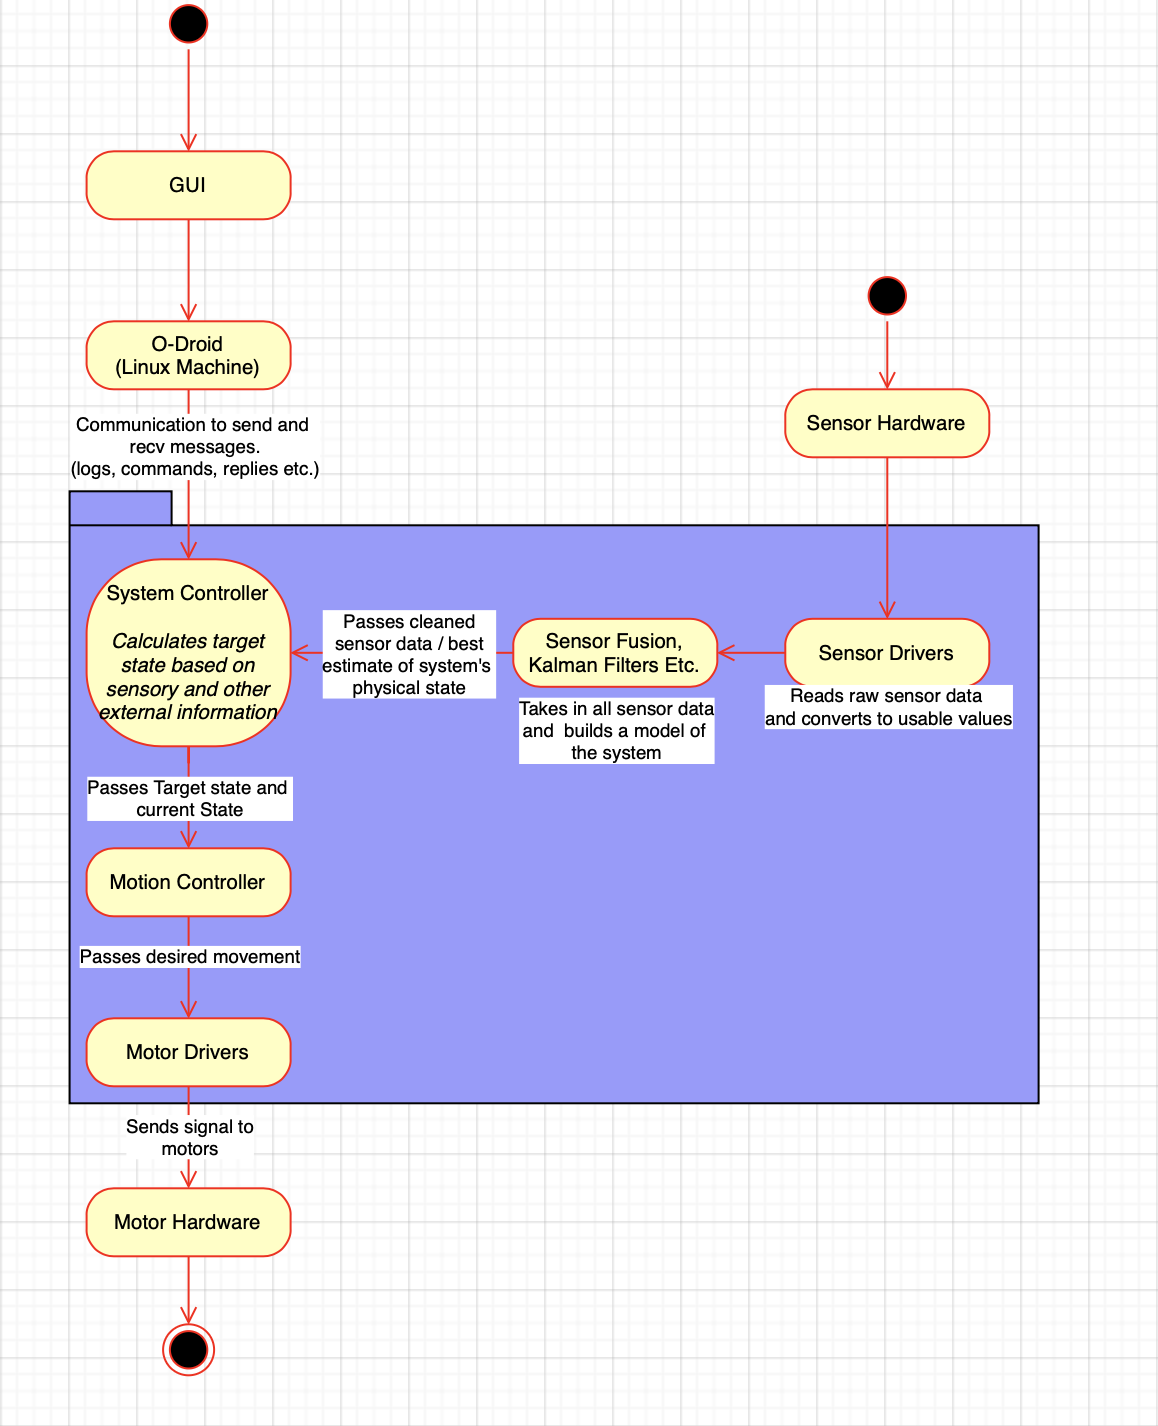
\includegraphics[scale=0.56]{./images/system_flow}
\end{figure}

\newpage
\subsection{External Message Flow Diagram}

\begin{figure}[h!]
\centering
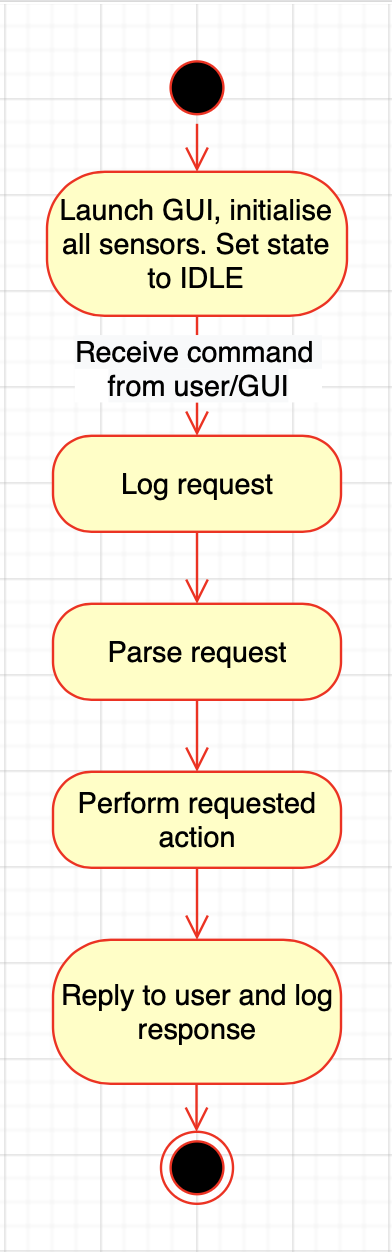
\includegraphics[scale=0.6]{./images/message_flow}
\end{figure}

\section{System Design}
This section describes the firmware design. This includes names for all required methods, functions and variables. In addition to naming, this section contains details of interfaces between subsystems.

\subsection{Class Diagram}

\begin{figure}[h!]
\centering
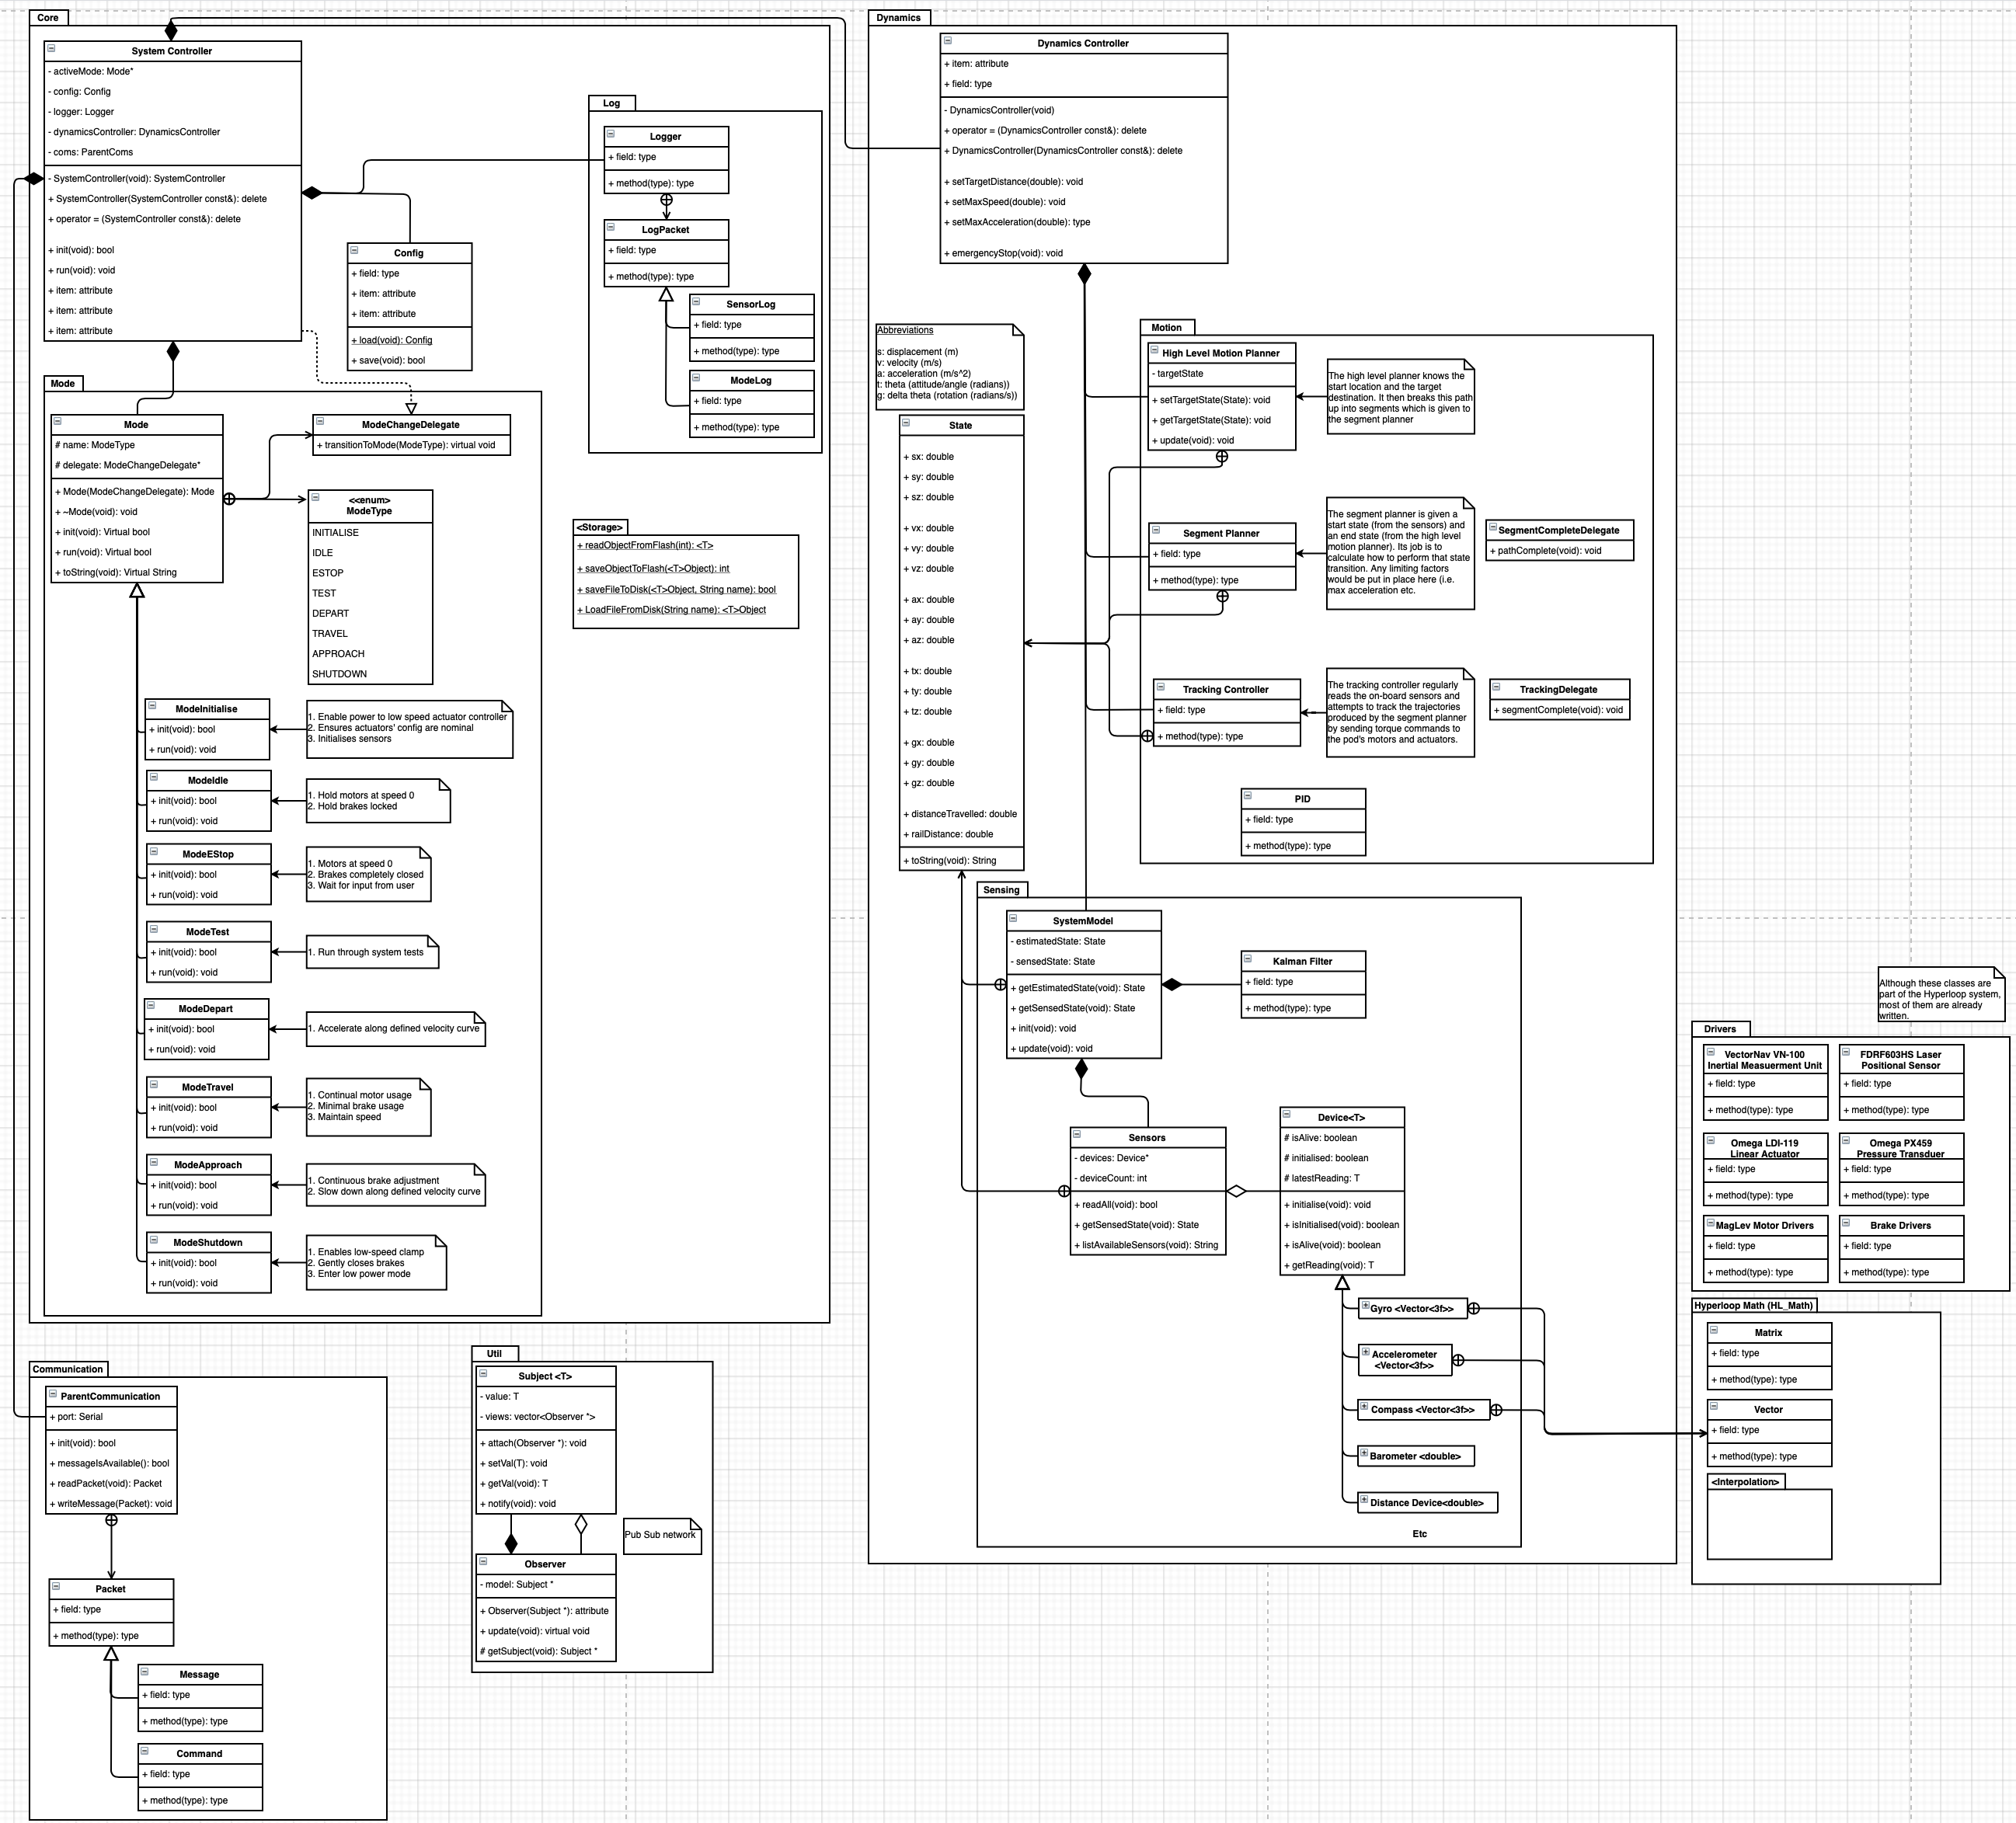
\includegraphics[scale=0.26]{./images/class_diagram}
\end{figure}

\section{Testing}

Every embedded system needs to be tested. Generally, it is also valuable or mandatory that testing be performed at several levels. The most common levels of testing are:

\begin{itemize}
    \item System tests verify that the product as a whole meets or exceeds the stated requirements. System tests are generally best developed outside of the engineering department, though they may fit into a test harness developed by engineers. \textbf{The system tests should treat the firmware as a black box.}
    
    \item Integration tests verify that a subset of the subsystems identified in the architecture diagrams interact as expected and produce reasonable outcomes. Integration tests are generally best developed by a testing group or person within software engineering.
    
    \item Unit tests verify that individual software components identified at the intermediate design level perform as their implementers expect. That is, they test at the level of the public API the component presents to other components. Unit tests are generally best developed by the same people that write the code under test. \textbf{Proponents of test-driven development advocate that tests at this level be written in advance of the functions or classes that they are intended to verify.}
\end{itemize}

Of the three, system tests are most easily developed, as those test the product at its exposed hardware interfaces to the world (e.g., does the dialysis machine perform as required). Of course, a test harness may need to be developed for engineering and/or factory acceptance tests. But this is generally still easier than integration and unit tests, which demand additional visibility inside the device as it operates.

To make the development, use, and maintenance of integration and unit tests easy, it is valuable to architect the firmware in a manner compatible with a software test framework. The single best way to do this is to architect the interactions between all software components at the levels you want to test so they are based on publish-subscribe event passing (a.k.a., message passing).

Interaction based on a publish-subscribe model allows a lightweight test framework like the one shown in Figure 2 to be inserted alongside the software component(s) under test. Any interface beween the test framework and the outside world, such as a serial port, provides an easy way to inject or log events. A test engine on the other side of that communications interface can then be designed to accept test “scripts” as input, log subscribed event occurrences, and off-line check logged events against valid result sequences. Adding timestamps to the event logger and scripting language features like delay(time) and waitfor(event) significantly increases testing capability.

\begin{figure}[h!]
\centering
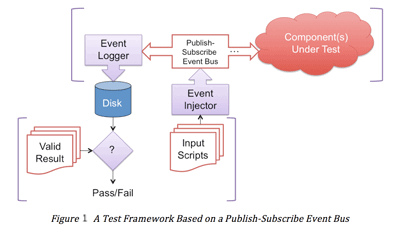
\includegraphics[scale=0.8]{./images/testing_procedure}
\end{figure}

It is unfortunate that the publish-subscribe component interaction model is at odds with proven methods of analyzing software schedulability (e.g., RMA). The sheer number of possible message arrival orders, queue depths, and other details make the analysis portion of guaranteeing timeliness difficult and fragile against minor implementation changes. This is, in fact, why it is important to separate the code that must meet deadlines from the rest of the software. In this architecture, though, the real-time functionality remains difficult to test other than at the system level.

\section{To Do}
To-do list for this document:
\begin{enumerate}
    \item Convert flow diagrams from images into compiled Latex
    \item Build out class diagrams
    \item Create architecture for O-Droid device
    \item Create class diagrams for O-Droid
    \item rewrite testing to make more sense in this specific application
\end{enumerate}

\end{document}
